\begin{figure}[t]
\centering
\begin{subfigure}{0.3\columnwidth}
	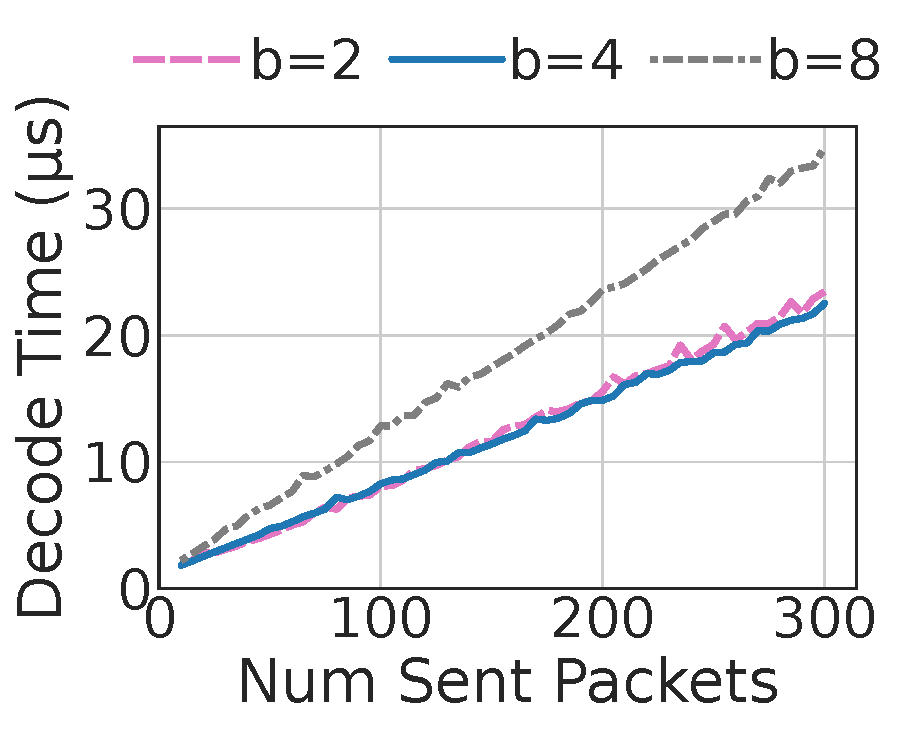
\includegraphics[width=\linewidth,trim={3mm 0 7mm 0},clip]{sidekick-paper/figures/fig2a_quack_num_candidates_vs_decode_time.pdf}
	\caption{Evaluate a degree-$m=t=10$ polynomial at $n$ candidate roots.}
	\label{fig:n-vs-decoding}
\end{subfigure}
\hspace{-0.1em}
\begin{subfigure}{0.32\columnwidth}
	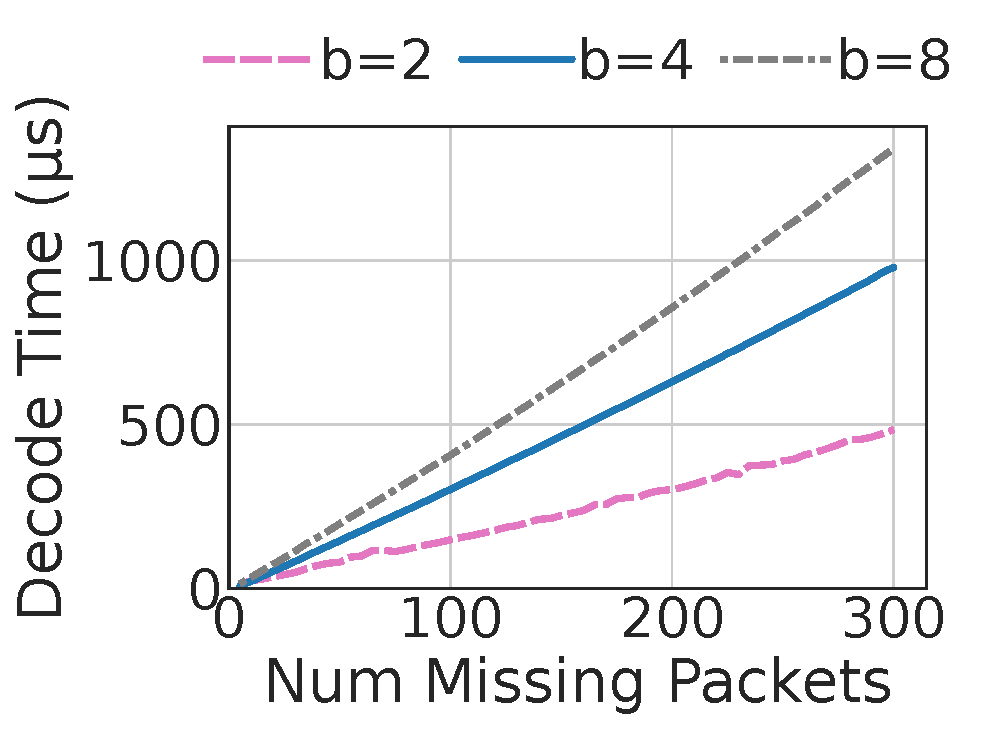
\includegraphics[width=\linewidth,trim={3mm 0 7mm 0},clip]{sidekick-paper/figures/fig2b_quack_num_missing_vs_decode_time.pdf}
	\caption{Plug $n=300$ candidate roots into a degree-$m$ polynomial.}
	\label{fig:m-vs-decoding}
\end{subfigure}
\hspace{-0.1em}
\begin{subfigure}{0.32\columnwidth}
	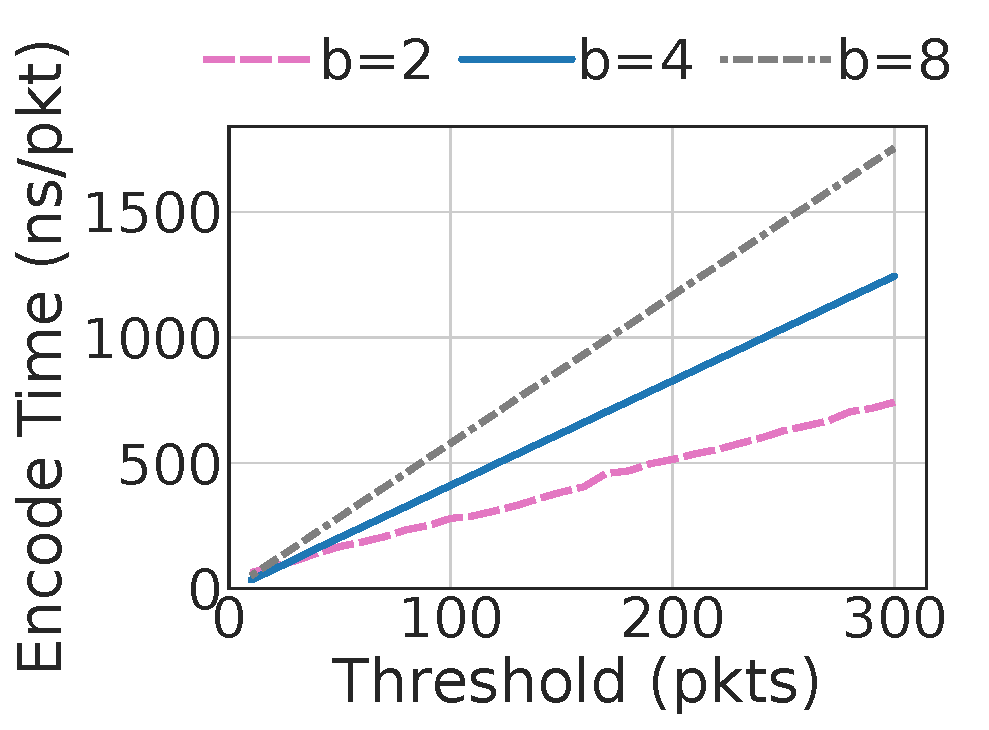
\includegraphics[width=\linewidth,trim={3mm 0 7mm 0},clip]{sidekick-paper/figures/fig2c_quack_threshold_vs_encode_time.pdf}
	\caption{Update $t$ power sum equations.
	Average of $1000$ packets.}
	\label{fig:construction-time}
\end{subfigure}
\caption{How power sum quACK performance depends on various parameters:
bit width, threshold, number of sent and missing packets.
Average of 100 trials.
}
\label{fig:quack-plots}
\end{figure}
